%%%%%%%%%%%%%%%%%%%%%%%%%%%%%%%%%%%%%%%%%%%%%%%%%%%%%%%%%%%%%%%%%%%%%%%%%%%%%%%%%%%%%%%%%%%%%%%%%%%%%%%%%%%%%%%%%%%%
%
% Masterarbeit im Fachbereich 1
% Systems Engineering - HTW Berlin
% 
% Thema:
% Lorem Ipsum
%
% \newcommand{\draftdate}{140910}
% \newcommand{\rev}{108}
% %
\newcommand{\thesisopening}{05. Januar 2015}
\newcommand{\thesisclosing}{16. März 2015}
\newcommand{\thesisrelease}{16. März 2015}
%%%%%%%%%%%%%%%%%%%%%%%%%%%%%%%%%%%%%%%%%%%%%%%%%%%%%%%%%%%%%%%%%%%%%%%%%%%%%%%%%%%%%%%%%%%%%%%%%%%%%%%%%%%%%%%%%%%%
%%%
%%
%





%%%%%%%%%%%%%%%%%%%%%%%%%%%%%%%%%%%%%%%%%%%%%%%%%%%%%%%%%%%%%%%%%%%%%%%%%%%%%%%%%%%%%%%%%%%%%%%%%%%%%%%%%%%%%%%%%%%%
%%%%%%%%%%%%%%%%%%%%%%%%%%%%%%%% D O K U M E N T K O N F I G U R A T I O N E N %%%%%%%%%%%%%%%%%%%%%%%%%%%%%%%%%%%%%
%%%%%%%%%%%%%%%%%%%%%%%%%%%%%%%%%%%%%%%%%%%%%%%%%%%%%%%%%%%%%%%%%%%%%%%%%%%%%%%%%%%%%%%%%%%%%%%%%%%%%%%%%%%%%%%%%%%%
%
%%
%%% 
% Dokumentformatierung
\documentclass
[a4paper,german,
12pt												% ersatzweise 12pt, wenn mehr Seiten entstehen sollen
]
{scrreprt}
%%%
%
%%%%%%%%%%%%%%%%%%%%%%%%%%%%%%%%%%%%%% P A C K A G E S %%%%%%%%%%%%%%%%%%%%%%%%%%%%%%%%%%%%%%%%%
%
%%% Textformatierung %%%
%

\usepackage[onehalfspacing]{setspace}				% Zeilenabstand bestimmen
\usepackage[table]{xcolor}							% farbiger Text
\usepackage{colortbl}								% Tabellen mit Hintergrundfarben versehen
\usepackage{lettrine}								% Kapitelbeginn mit großem Buchstaben
\usepackage{fancybox}								% Schattierungen und Rahmen für Grafiken
\usepackage{wrapfig}								% Paket zur Positionierung von Grafiken
\usepackage{capt-of}								% Untertitel von Abbildungen, Tabellen usw. in Gleitumgebung
\usepackage[ngerman]{babel,translator}				% Silbentrennung nach der neuen deutschen Rechtschreibung, z.B.: Sys-tem
\usepackage{paralist}								% Kompakte Aufzaehlungen erstellen
\usepackage[bottom]{footmisc}							% Fussnoten am Seitenende
\usepackage{fancyhdr}								% Kopf- und Fußzeilenformatierung
\usepackage{pdfpages}								% für die Einbindung kompletter pdf-*Seiten*
\usepackage{eso-pic}								% Wasserzeichen z.B. "`ENTWURF"' auf .pdf erzeugen
\usepackage[hyphens]{url}							% für \url{http://www}, Option hyp erlaubt auch Umbruch nach "-"
\usepackage[numbers,square]{natbib}					% Für \setlength{\bibsep}{3mm}; square macht eckige Klammern
\usepackage{bibgerm}								% Styles für Literaturverzeichnisse
\usepackage{titlesec, blindtext, color}				% Styles für Kapitelüberschriften
\usepackage[printonlyused,withpage]{acronym}		% Abkürzungsverzeichnis
%
\usepackage{tabularx}
\usepackage[utf8]{inputenc}							% Zeichensatz, ermöglicht die direkte Eingabe von Umlauten im Editor
\usepackage[T1]{fontenc}							% Optimiert Umlautverwendung
\usepackage{lmodern}								% Schriften aufgrund von 'fontenc' glätten
\usepackage{graphicx}								% Einbindung von Grafiken (pdf, png, jpg)
\usepackage{float}									% bietet Option [H] für bombenfestes Verankern
\usepackage{enumerate}								% verbessert Aufzählungen
\usepackage{expdlist}								% erweiterter Funktionssatz für description
\usepackage{chngcntr}								% Konfiguration des Fußnotenzählers ermöglichen
\usepackage{array}									% für Tabellen: bindet tabular-Umgebung ein
\usepackage{parskip}								% zw. Absätzen: eine knappe Leerzeile statt hängender Einzüge
\usepackage[right]{eurosym}							% Eurosymbol
\usepackage{makeidx}								% Package zur Indexerstellung
\usepackage{multicol}								% zur Indexerstellung in zwei Spalten
\usepackage{multirow}								% Verbinden von Zellen in Tabellen
\usepackage{booktabs}								% Tabellenlayout anpassen
\usepackage{longtable}								% Tabellen über mehrere Seiten strecken
\usepackage{chngcntr}								% Nummeriegung der Abbildungen beeinflussen (z.B. nach Kapitel/fortlaufend)
\usepackage[outercaption]{sidecap}					% Bildunterschriften rechts neben der Abbildung positionieren
\usepackage[bf]{caption}							% Kuerzel und Nummerierung von Bildunterschriften "`fett"' schreiben
\usepackage{amssymb}								% Erweiterte Symboldarstellung
\usepackage{times}
\usepackage{listings}
%%
% Packagehinweise
% Folgende Packete müssen zusätzlich von MiKTeX bereitgestellt werden:
% setspace, xcolor, colortbl, lettrine, fancybox, wrapfig, capt-of, translator, paralist, expdlist, footmisc, fancyhdr, pdfpages, eso-pic, url,
% natbib, bibgerm, titlesec, blindtext, acronym, suffix, xstring, glossaries, etoolbox, textcase, xfor, datatool-base, substr, fp, supertabular,
% mptopdf
%%
%%%%%%%%%% NEW FOR TESTING %%%%%%%%%%
%
%%


%%LISTINGS SETTINGS
\definecolor{mygreen}{rgb}{0,0.6,0}
\definecolor{mygray}{rgb}{0.5,0.5,0.5}
\definecolor{mymauve}{rgb}{0.58,0,0.82}


\lstset{ %
  backgroundcolor=\color{white},   % choose the background color; you must add \usepackage{color} or \usepackage{xcolor}
  basicstyle=\footnotesize,        % the size of the fonts that are used for the code
  breakatwhitespace=false,         % sets if automatic breaks should only happen at whitespace
  breaklines=true,                 % sets automatic line breaking
  captionpos=b,                    % sets the caption-position to bottom
  commentstyle=\color{mygreen},    % comment style
  deletekeywords={...},            % if you want to delete keywords from the given language
  escapeinside={\%*}{*)},          % if you want to add LaTeX within your code
  extendedchars=true,              % lets you use non-ASCII characters; for 8-bits encodings only, does not work with UTF-8
  frame=single,                    % adds a frame around the code
  keepspaces=true,                 % keeps spaces in text, useful for keeping indentation of code (possibly needs columns=flexible)
  keywordstyle=\color{blue},       % keyword style
  language=C++,                 % the language of the code
  morekeywords={*,...},            % if you want to add more keywords to the set
  numbers=left,                    % where to put the line-numbers; possible values are (none, left, right)
  numbersep=5pt,                   % how far the line-numbers are from the code
  numberstyle=\tiny\color{mygray}, % the style that is used for the line-numbers
  rulecolor=\color{black},         % if not set, the frame-color may be changed on line-breaks within not-black text (e.g. comments (green here))
  showspaces=false,                % show spaces everywhere adding particular underscores; it overrides 'showstringspaces'
  showstringspaces=false,          % underline spaces within strings only
  showtabs=false,                  % show tabs within strings adding particular underscores
  stepnumber=2,                    % the step between two line-numbers. If it's 1, each line will be numbered
  stringstyle=\color{mymauve},     % string literal style
  tabsize=2,                       % sets default tabsize to 2 spaces
  title=\lstname                   % show the filename of files included with \lstinputlisting; also try caption instead of title
}
%%% Abstellgleis %%%
%
%Options: Sonny, Lenny, Glenn, Conny, Rejne, Bjarne, Bjornstrup
%\usepackage[Glenn]{fncychap}
%%
%%% Referenzierung / Dokumentenlinks %%%
% LINK packages IMMER zuletzt einbinden!!!
\usepackage{hyperref}			% Package für Textlinks in pdf-Datei / Option [colorlinks] färbt Text rot!
\usepackage[toc,nonumberlist,nopostdot]{glossaries}	% Automatisches Glossar erstellen
%%%
%
%%%%%%%%%%%%%%%%%%%%%%%%%%%%%% W A S S E R Z E I C H E N %%%%%%%%%%%%%%%%%%%%%%%%%%%%%%%%%%%%%%%
%
\AddToShipoutPicture{%
    \AtTextCenter{%
      \makebox(0,0)[c]{\resizebox{\textwidth}{!}{%
        \rotatebox{45}{\textsf{\textbf{\color{lightgray}DRAFT//\draftdate}}}}} 
    }
  }
\ClearShipoutPicture
%%%
%
%%%%%%%%%%%%%%%%%%%%%%%%%%%%%%%%%%%%%%%% D E F I N E %%%%%%%%%%%%%%%%%%%%%%%%%%%%%%%%%%%%%%%%%%%
%


\definecolor{darkred}{rgb}{0.7,0.0,0.0}				% Textfarben definieren
\definecolor{hellgrau}{rgb}{0.95,0.95,0.95}
\definecolor{dunkelgrau}{rgb}{0.8,0.8,0.8}
\sloppy												% großzügiger Zeilenumbruch -> keine rechts rausragenden Zeilen mehr
%
\def\TReg{\textsuperscript{\textregistered}}
\def\TCop{\textsuperscript{\textcopyright}}
\def\TTra{\textsuperscript{\texttrademark}}
%
\newcommand{\ctab}{\centering\arraybackslash}		% Text in Tabellenzellen zentrieren
\newcolumntype{C}[1]{>{\centering\arraybackslash}p{#1}} % Text spaltenweise zentrieren
%
% Abstand zwischen Nummerierung und Text veraendern
\makeatletter
\renewcommand*\l@figure{\@dottedtocline{1}{1.5em}{3em}}
\renewcommand*\l@table{\@dottedtocline{1}{1.5em}{3em}}
\makeatother
%
% Farben fuer Verknuepfungen/Verweise anpassen
\hypersetup{
	linktocpage			= true,
	colorlinks			= true,
	linkcolor			= black,
	citecolor			= green,
	filecolor			= magenta,
	urlcolor			= cyan,
	pdftitle			= {Thesis M. Musterfrau},
	pdfauthor			= Monika Musterfrau,
	pdfsubject			= {Untersuchungen zum Vernetzen der Netze},
	pdfdisplaydoctitle	= true,
%	bookmarks			= true,
	bookmarksnumbered	= true,
	pdfpagemode			= UseOutlines,
	pdfpagelayout		= SinglePage,
	pdfprintscaling		= None,
}
%%%
%
%%%%%%%%%%%%%%%%%%%%%%%%%%%%%%%%%%%%% F O O T N O T E S %%%%%%%%%%%%%%%%%%%%%%%%%%%%%%%%%%%%%%%%%
% Fortlaufende Fußnoten (regulär wird der Zähler zu Beginn eines neuen Kapitels zurückgesetzt)
%
\counterwithout{footnote}{chapter}
%%%
%
%%%%%%%%%%%%%%%%%%%%%%%%%%%%%%%%%%%%%% C A P T I O N S %%%%%%%%%%%%%%%%%%%%%%%%%%%%%%%%%%%%%%%%%%
%
% Beschriftung für Abbildungen und Tabellen formatieren
\addto\captionsngerman{\renewcommand\figurename{Abb.}}
\addto\captionsngerman{\renewcommand\tablename{Tab.}}
\counterwithin{figure}{section}
\counterwithin{table}{section}
%%%
%
%%%%%%%%%%%%%%%%%%%%%%%%% L I T E R A T U R V E R Z E I C H N I S %%%%%%%%%%%%%%%%%%%%%%%%%%%%%%
%
% Literaturverzeichnis mit BibTeX
%
\bibliographystyle{alphadin}						% 
\setlength{\bibsep}{3mm}							% Abstände im Literaturverzeichnis
%%%
%
%%%%%%%%%%%%%%%%%%%%%%%%%%%%%%% K O P F - & F U ß Z E I L E %%%%%%%%%%%%%%%%%%%%%%%%%%%%%%%%%%%%
%
% Größenanpassungen
%
\setlength{\headheight}{16pt}						% Höhe der Kopfzeile anpassen
\setlength{\unitlength}{1cm}
\setlength{\oddsidemargin}{0.3cm}
\setlength{\evensidemargin}{0.3cm}
\setlength{\textwidth}{16.5cm}
\setlength{\topmargin}{-1.2cm}
\setlength{\textheight}{24.5cm}
\columnsep 0.5cm
%%%
%
%%%%%%%%%%%%%%%%%%%%%%%%%%%% I N H A L T S V E R Z E I C H N I S %%%%%%%%%%%%%%%%%%%%%%%%%%%%%%%
%
% Strukturtiefe des Inhaltsverzeichnis
%
\setcounter{secnumdepth}{5}
\setcounter{tocdepth}{5}
%%%
%
%%%%%%%%%%%%%%%%%%%%%%%%%%%%%% T R E N N U N G S R E G E L N %%%%%%%%%%%%%%%%%%%%%%%%%%%%%%%%%%%
%
% Anmerkung: für Wörter mit Umlauten muss das Paket \usepackage[T1]{fontenc} eingebunden werden --
% in der vorliegenden Version funktionieren *keine* Umlaute!!
% 
\hyphenation{}
%%%
%
%%%%%%%%%%%%%%%%%%%%%%%%%%%%%%%%%%% G L O S S A R %%%%%%%%%%%%%%%%%%%%%%%%%%%%%%%%%%%%%%%%%%%%%%
%
%\loadglsentries{glossary/glossary}					% Externes Glossarverzeichnis laden
\makeglossaries										% Aufruf zur automatischen Erstellung des Glossars
%%%
%
%%%%%%%%%%%%%%%%%%%%%%%%% T E X T F L U S S - P A R A M E T E R %%%%%%%%%%%%%%%%%%%%%%%%%%%%%%%%
%
\clubpenalty = 10000 
\widowpenalty = 10000
\displaywidowpenalty = 10000
\interlinepenalty = 5000							% u.a. sauberen Umbruch bei Eintraegen in Verzeichnissen!
%%%
%%
%
%%%%%%%%%%%%%%%%%%%%%%%%%%%%%%%%%%%%%%%%%%%%%%%%%%%%%%%%%%%%%%%%%%%%%%%%%%%%%%%%%%%%%%%%%%%%%%%%%%%%%%%%%%%%%%%%%%%%
%%%%%%%%%%%%%%%%%%%%%%%%%%%%%%%%%%%%%% D O K U M E N T E R S T E L L U N G %%%%%%%%%%%%%%%%%%%%%%%%%%%%%%%%%%%%%%%%%
%%%%%%%%%%%%%%%%%%%%%%%%%%%%%%%%%%%%%%%%%%%%%%%%%%%%%%%%%%%%%%%%%%%%%%%%%%%%%%%%%%%%%%%%%%%%%%%%%%%%%%%%%%%%%%%%%%%%
%
%%
%%%




\begin{document}
%%%
%
%%%%%%%%%%%%%%%%%%%%%%%%%%%%%%% I N L I N E T I T L E P A G E %%%%%%%%%%%%%%%%%%%%%%%%%%%%%%%%%%
% Dokumentinformationen zur automatischen Erstellung einer Titelseite
% Ist nur erforderlich, wenn keine eigenständige Titelseite eingebunden wird!

%\title{TEST}										% Legt den Titel des Dokuments fest
%\author{M. Musterfrau  }							% Angabe über den/die Autor(en)
%\date{\today}										% Liefert das aktuelle Datum bei Dokumenterstellung
% maketitel											% Aufruf zum Erstellen und Einbinden der Titelseite
%%%
%
%%%%%%%%%%%%%%%%%%%%%%%%%%%%%%%%%%%% T I T E L S E I T E %%%%%%%%%%%%%%%%%%%%%%%%%%%%%%%%%%%%%%%
% Beginn der ersten Seite im Dokument
%
\pagenumbering{Alph}								% Formatierung der Seitennummerierung auf große Buchstaben
%
\include{01_Titel}
%%%
%
%%%%%%%%%%%%%%%%%%%%%%%%%%%%%%%%%%%%%% V O R S P A N N %%%%%%%%%%%%%%%%%%%%%%%%%%%%%%%%%%%%%%%%%
%
\clearpage \setcounter{page}{-1}						% Start der Seitennummerierung, da Titelseite ohne Seitenzahl
%
\chapter*{Eidesstattliche Erklärung}
\label{chapter_erklaerung}
\thispagestyle{empty}

\vfill

Tim Nieter\\
Rudower Straße 95\\
12351 Berlin

\vspace{\baselineskip}

Hiermit versichere ich, dass ich die von mir vorgelegte Arbeit selbstständig verfasst habe, dass ich die verwendeten Quellen und Hilfsmittel
 vollständig angegeben habe und dass ich die Stellen der Arbeit -- einschließlich Tabellen und Abbildungen --, die anderen Werken oder dem Internet im
 Wortlaut oder dem Sinn nach entnommen sind, auf jeden Fall unter Angabe der Quelle als Entlehnung kenntlich gemacht habe.

\vspace{\baselineskip}

Berlin, den {16. März 2015}

\vspace{1cm}

Tim Nieter

\vspace{.5cm}

\underline{~~~~~~~~~~~~~~~~~~~~~~~~~~~~~~~~~~~~~~~~}\\
(Unterschrift)


%
\chapter*{Sperrvermerk}
\label{chapter_sperrvermerk}
\thispagestyle{empty}

Die nachfolgende Bachelorarbeit mit dem Titel \glqq Entwicklung eines vollautomatisierten Embedded-Linux-Systems zur Ansteuerung und Auswertung eines Langzeittests\grqq\ enthält
vertrauliche Daten der Pepperl+Fuchs GmbH. Veröffentlichungen oder Vervielfältigungen der
Arbeit – auch nur auszugsweise – sind ohne ausdrückliche Genehmigung der Pepperl+Fuchs GmbH
nicht gestattet. Die Arbeit ist lediglich den Korrektoren sowie den Mitgliedern
der Prüfungskommission zugänglich zu machen.




\thispagestyle{empty}


{\large \textbf{Tim Nieter}}\\

{\large \textbf{Thema der Bachelorarbeit}}\\
Entwicklung eines vollautomatisierten Embedded-Linux-Systems zur Ansteuerung und Auswertung eines Langzeittests.\\

{\large \textbf{Stichworte}}\\
BeagleBone Black, Qt, MySQL\\

{\large \textbf{Kurzzusammenfassung}}\\
Im Rahmen dieser Arbeit wird eine Embedded-Linux-System unter Verwendung eines Einplatinencomputers zur Ansteuerung und Auswertung eines Langzeittests entwickelt. Des Weiteren wird zur Erfassung von Messdaten ein RS232 Protokoll und ein MySQL Datenbanksystem implementiert werden. Für die Auswertung und Verwaltung der Daten wird eine Ethernet Schnittstelle und ein Webinterface gestaltet.
% 
\clearpage											% Wechsel auf die nächste freie Seite
\pagenumbering{Roman}								% Seitenzahlen auf große römische Zahlen setzen
\setcounter{page}{0}								% Fortfahren mit Seitenzahl des letzten Abschnitts
%%%
%
%%%%%%%%%%%%%%%%%%%%%%%%%%%%%%%%% V E R Z E I C H N I S S E %%%%%%%%%%%%%%%%%%%%%%%%%%%%%%%%%%%%%
%
%%% Anfang des Inhaltsverzeichnisses
\pdfbookmark{Inhaltsverzeichnis}{toc}				% Bookmark zum Inhaltsverzeichnis
\tableofcontents
\clearpage
%
%%% Anfang des Abbildungsverzeichnisses
\listoffigures
\protect \addcontentsline{toc}{chapter}{Abbildungsverzeichnis}
\clearpage
%
%%% Anfang des Tabellensverzeichnisses
\listoftables
\protect \addcontentsline{toc}{chapter}{Tabellenverzeichnis}
\clearpage


\renewcommand{\lstlistingname}{Quellcode}% Listing -> Algorithm
\renewcommand{\lstlistlistingname}{\lstlistingname verzeichnis}% List of Listings -> List of Algorithms


\lstlistoflistings
\protect \addcontentsline{toc}{chapter}{Quellcodeverzeichnis}
\clearpage

%
%%% Anfang des Abkürzungsverzeichnis
\phantomsection \addcontentsline{toc}{chapter}{Abkürzungsverzeichnis}
\renewcommand\refname{Abkürzungsverzeichnis} \chapter*{Abkürzungsverzeichnis}






%\renewcommand*\bflabel[1]{\textbf{#1}\hfill}
%
% Abkürzungsverzeichnis

\begin{acronym}[MySQL]
\acro{SQL}{Structured Query Language}
\acro{DB}{Datenbank}
\acro{DBMS}{Datenbankmanagementsystem}
\acro{DBS}{Datenbanksystem}
\acro{ER}{Entity-Relationship}
\acro{ERM}{Entity-Relationship-Modell}
\acro{DUT}{Device Under Test}
\acrodefplural{DUT}[DUTs]{Devices Under Test}
\acro{GUI}{Graphical User Interface}
\acro{IDE}{Integrated Developement Environment}
\acro{SDK}{Software Developement Kit}
\acro{LED}{Light-Emitting Diode}
\acro{ADC}{Analog-Digital-Converter}
\acro{LTT}{Long Term Test}
\acro{UART}{Universal Asynchronous Receiver Transmitter}
\acro{BBB}{BeagleBone Black}
\end{acronym}

%
\clearpage
%
%%% Glossarverzeichnis
\glsaddall
\printglossary[style=altlisthypergroup]
\clearpage
%%%
%
%%% Änderungshistorie
%\input{basix/history}
%%%
%
%%%%%%%%%%%%%%%%%%%%%%%% S E I T E N L A Y O U T  E I N S T E L L E N %%%%%%%%%%%%%%%%%%%%%%%%%%%%%
%
\clearpage \pagenumbering{arabic}					% Seitenzahlen zurücksetzen und Formatierung auf Arabisch
%

\pagestyle{fancy}									% Eigenen Seitenstil aktivieren
%
\renewcommand{\chaptermark}[1]{\markboth{\uppercase{\thechapter\ #1}}{}}
\renewcommand{\sectionmark}[1]{\markright{\thesection\ #1}}
\lhead{\slshape \nouppercase \leftmark }
\chead{}
\rhead{\slshape \nouppercase \rightmark }
\lfoot{}
\cfoot{\thepage}
\rfoot{}
\renewcommand{\headrulewidth}{0.4pt}
\renewcommand{\footrulewidth}{0pt}

%%%
%

%%%%%%%%%%%%%%%%%%%%%%%%%%%%%%%%%%%%%%%%%%%%%%%%%%%%%%%%%%%%%%%%%%%%%%%%%%%%%%%%%%%%%%%%%%%%%%%%%%%%%%%%%%%%%%%%%%%%
%%%%%%%%%%%%%%%%%%%%%%%%%%%%%%%%%%%% BEGINN der wissenschaftlichen Arbeit %%%%%%%%%%%%%%%%%%%%%%%%%%%%%%%%%%%%%%%%%%
%%%%%%%%%%%%%%%%%%%%%%%%%%%%%%%%%%%%%%%%%%%%%%%%%%%%%%%%%%%%%%%%%%%%%%%%%%%%%%%%%%%%%%%%%%%%%%%%%%%%%%%%%%%%%%%%%%%%
%
%%
%%%

\chapter{Einleitung}
\label{chapter_einleitung}
In diesem ersten Kapitel wird auf die Motivationen und die Zielsetzung dieser Arbeit eingegangen.

\section{Motivation}
Wann immer Systeme in der realen Welt eingesetzt werden, sollen sie so zuverlässig, fehlerfrei und vorhersehbar wie möglich arbeiten. Gerade wenn diese Systeme an kritischen Punkten zum Einsatz kommen und über lange Zeiträume agieren, sind diese Eigenschaften besonders wichtig.\\
Um diesen Anforderungen gerecht zu werden, müssen alle Bauelemente eines solchen Systems diese Vorgaben erfüllen, denn die Zuverlässigkeit ist immer abhängig vom schwächsten Glied.
Bei der Entwicklung eines Systems ist es somit entscheidend, alle Bauelemente vorher anhand der gegebenen Umstände zu qualifizieren. Dafür müssen die Grenzen ausgelotet werden, in denen sie zuverlässig betrieben werden können.

Eine dieser Grenzen ist die altersbedingte Änderung der Betriebsparameter, die sogenannte Degradation.
Um das Degradationsverhalten eines Bauelementes bestimmen zu können, muss es über lange Zeiträume unter erschwerten Bedingungen betrieben und ausgewertet. Nur wenn ein Bauelement ein für die Anwendung akzeptables Degradationsverhalten aufweist, ist es für den Einsatz im Gesamtsystem geeignet.\\
Da ein hoher Einsatz von Ressourcen nötig ist, um jedes Bauelement individuell zu Prüfen, existieren automatisierte Teststände mit deren Hilfe der Aufwand minimiert werden soll.
 

\section{Szenario und Zielsetzung}
Ein Unternehmen stellt verschiedene optoelektronischen Sensoren her. Zur Sicherstellung der Zuverlässigkeit der verwendeten \ac{LED} sollen diese mittels eines automatisierten Teststandes bezüglich ihre Degradationsverhaltens überprüft werden.\\
Aus diesem Grund soll im Rahmen dieser Arbeit ein solcher Teststand entwickelt werden. Das beinhaltet die Datenerfassung, die Datenauswertung und die Überwachung des Systems. 
\chapter{Grundlagen}
\label{chapter_Grundlagen}

Bei der Entwicklung des Teststandes kommen verschiedene Systeme und Konzepte zum Einsatz. Dieses Kapitel befasst sich mit der C++ Klassenbibliothek Qt und der Frage, was ist die Degradation oder ein Embedded-Linux-System. Des Weiteren wird auf das Konzept einer Datenbank und der Evaluierung der beiden Datenbanksysteme MySQL und SQLite eingegangen.

\section{Degradation}
\label{section_Degradation}
Der Hauptgrund für mechanisches Versagen im Lebenszyklus eines Systems oder Bauelementes, liegt an der langsamen Ansammlung von nicht reversiblen Schäden. Dieser Prozess ist bekannt als Degradation (vgl. \cite{zhou2011}).\\
Die Schwierigkeit liegt in der Feststellung des mechanischen Versagens in messbaren Schritten.\\
So ist die Bestimmung der Lebenszeit über die Zeit bis zum Ausfall zeitaufwändig. Einfacher ist es die Leistung des Bauelementes oder Systems zu erfassen, z.B. die optische Leistung einer \ac{LED}. Auf diesem Weg kann ein Trend ausgemacht werden.\\
Um die Länge des Lebenszyklus eines Bauelementes bestimmen zu können, wird die Leistung dessen unter Last über einen langen Zeitraum hinweg aufgezeichnet. Anhand der daraus resultierenden Daten kann die zu erwartende Länge des Lebenszyklus ermittelt werden.\ 

In Abbildung \ref{figure_Degradation} ist ein Beispiel für erfasste Daten zu sehen. Sie zeigt die relative Abweichung der optischen Leistung über die Zeit von sieben verschiedenen \acp{LED}. Bei den durch die rote und braune Kurve repräsentierten \acp{LED} dürfte nach den hier vorliegenden Messergebnissen nicht davon ausgegangen werden, dass nach 20.000 Stunden mehr als 70\% der ursprünglichen Lichtleistung vorhanden ist. Dagegen deuten die grünen Kurve bereits nach 5.000 Stunden auf eine sehr hohe Lebenserwartung der entsprechenden LEDs hin. Diese Aussagen können nur getroffen werden, da über einen sehr langen Zeitraum Messungen in sehr kurzem Abstand erfasst wurden.

 
\begin{figure}[H]
\begin{center}
\includegraphics[width=0.8\textwidth]{img/general/DegradationMin.png}
\caption{Aufgezeichnete Degradation}
\label{figure_Degradation}
\end{center}
\end{figure}



\section{Qt}
\label{section_Qt}
Qt \cite{qtproject} ist eine umfangreiche C++-Klassenbibliothek zur Gestaltung und Entwicklung von Anwendungen. Vor allem bei Applikationen mit grafischen Benutzeroberflächen (englisch: \ac{GUI}) ist Qt sehr beliebt. \\
Zusätzlich bringt Qt eine große Auswahl an Tools und Modulen mit sich, welche die Programmierung erheblich erleichtern (z.B. Netzwerkprogrammierung, Datenbankanbindung, OpenGL, etc.). \\
Ein weiterer Vorteil ist die Plattformunabhängigkeit. So unterstützt Qt aktuell (Version 5.4, 10. Dezember 2014) einen Großteil der aktuellen Betriebssysteme wie Windows, Linux, Android, iOS und einige mehr. Die hohe Kompatibilität wird dadurch gegeben, dass Qt die meisten Systemaufrufe abstrahiert.

\subsection{Signale und Slots}
\label{QtSignaleSlots}
Die Kommunikation unter den Objekten in Qt erfolgt über Signale und Slots. Dabei sendet ein Objekt ein Signal aus und ein anderes empfängt dieses. Dafür muss zunächst eine Verbindung zwischen den Objekten aufgebaut werden. Das erfolgt mit dem \textit{connect}-Statement.\\

\begin{lstlisting}[caption={Qt \textit{connect}-Statement},label=lst_QtConnect]
connect(Calculate, SIGNAL(clicked()), this, SLOT(addAB()));
\end{lstlisting}

Im Quellcode \ref{lst_QtConnect} wird ein Beispiel für die Verbindung von zwei Objekten mit dem \textit{connect}-Statement gezeigt. Hier wird das Signal \textit{clicked()} des Objektes \textit{Calculate} mit dem Slot \textit{addAB()} des Objektes \textit{this}, was dem aktuellen Objekt entspricht, verbunden. \\

\begin{lstlisting}[caption={Qt \textit{emit}-Statement},label=lst_QtEmit]
void Calculate::my_function(){
	/*
	Do Something
	*/
	emit clicked();	
}
\end{lstlisting}

Im Quellcode \ref{lst_QtEmit} wird das Signal \textit{clicked()} nun mittels \textit{emit}-Statement ausgelöst und der Slot des verbundenen Objektes aktiviert. Dadurch wird die Funktion \textit{addAB()} ausgeführt. Somit ist es möglich beispielsweise die GUI und den Hauptprogrammablauf von einander zu trennen und lediglich über Signale und Slots kommunizieren zu lassen. Beide Programmteile agieren dabei komplett unabhängig von einander.

\subsection{Entwicklungsumgebung}
Als Entwicklungsumgebung (englisch: \ac{IDE}) dient der Qt Creator (siehe Abbildung \ref{QtCreator}), welcher Teil des \ac{SDK} von Qt ist und sowohl für Linux, Windows als auch Mac OS X zur Verfügung steht. Er kommt mit einem Debugger, einem integrierten \ac{GUI} Designer und einem Texteditor, welcher unter anderem Funktionen wie Syntax-Hervorhebung und automatischer Vervollständigung beherrscht. \\
Dabei kommen gängige Compiler wie MinGW unter Windows zum Einsatz und es besteht die Möglichkeit eigene Toolchains anzulegen. \\
Eine Toolchain dient zum Übersetzen von Quellcode auf einem Host-System für ein Ziel-System. Sie setzt sich meistens aus einer Kette (englisch: chain) von Werkzeugen (englisch: tool) zusammen, welche nacheinander für die Übersetzung des Quellcodes sorgen. Somit ist es möglich, einen Programmcode auf einem Windowsrechner zu schreiben und anschließend für ein Linux-System zu übersetzen.

\begin{figure}[H]
\begin{center}
\includegraphics[width=0.8\textwidth]{img/general/QtCreator.png}
\caption{QtCreator Version 2.0.1 (Quelle: \protect\cite{qtcreator})}
\label{QtCreator}
\end{center}
\end{figure}

%Quellen:\\
%http://de.wikipedia.org/wiki/Qt_%28Bibliothek%29
%http://www.mathematik.uni-ulm.de/sai/ws02/cpp/070103/Qt.pdf
%http://wiki.ubuntuusers.de/Qt
%http://en.wikipedia.org/wiki/Qt_Creator


\section{Datenbank}
\label{section_Datenbank}

Um große Mengen an Daten effizient verarbeiten zu können, ist der Einsatz eines \ac{DBMS} ratsam (vgl. \citep{saake2010datenbanken}).

Für das Speichern von Daten und Betriebsparametern wird daher eine \ac{SQL} \ac{DB} benötigt. Bei der Wahl des \ac{DBMS}, stehen mehrere Systeme zur Auswahl. Dabei kommen SQLite und MySQL aufgrund der kostenlosen Verfügbarkeit in die engere Auswahl.
Beide System haben ihre Vor- und Nachteile.


\textbf{SQLite} ist ein \ac{SQL} \ac{DBMS}, welches ohne einen Server auskommt und operiert stattdessen in einer einzigen Datei. Alle Informationen wie Tabellenstruktur und Daten sind darin enthalten. Es wird vor allem im eingebetteten Bereich eingesetzt, da kaum Konfigurationen oder Verwaltung notwendig sind. Deshalb eignet es sich ausgezeichnet für sich schnell weiterentwickelnde Applikationen.
\\
Aufgrund dieser Eigenschaften existieren allerdings auch Nachteile. So unterstützt SQLite nur eingeschränkt mehrere Nutzer, die gleichzeitig auf die Datenbank zugreifen. Da das gesamte \ac{DBS} in einer einzigen Datei zusammengefasst ist, können mehrere zur selben Zeit durchgeführte Schreibzugriffe nicht unterstützt werden. Denn die einzige Zugriffskontrolle und Sicherstellung der Datenintegrität erfolgt durch das Dateisystem des Betriebssystem, was nicht immer fehlerfrei implementiert ist.
\\
Des Weiteren ist SQLite aufgrund des Ein-Datei-Systems nur eingeschränkt skalierbar. Bei einer größeren Datenmenge oder erhöhten Anzahl an Zugriffen ist es nicht möglich diese Datei auf mehrere Systeme zu separieren, um somit die Last gleichmäßig zu verteilen.

\textbf{MySQL} ist ein weiteres \ac{SQL} \ac{DBMS}, welches allerdings auf einer Serverarchitektur beruht. 
Es ermöglicht die Verwaltung von Nutzern und Rechten. Dadurch ist es ausgezeichnet für den gleichzeitigen Zugriff mehrerer Nutzer geeignet.\\ Außerdem ist das System gut hinsichtlich Performance und Größe zu skalieren, da die Last auf mehrere Server verteilbar ist. Zusätzlich bietet MySQL viele weitere Möglichkeiten für Performanceoptimierung, wie z.B. Query-Caching. Beim Query-Caching werden Ergebnisse von SQL-Abfragen (englisch: SQL-Query) zwischengespeichert, so dass sie bei erneuter Abfrage bereits vorliegen.
\\
Jedoch gibt es auch hier Nachteile. So ist die Konfiguration wesentlich schwerer und komplexer. Während bei SQLite kaum Konfigurationen nötig sind, müssen bei MySQL viele Einstellungen an das Host-System angepasst werden. Darunter fallen beispielsweise verschiedene Zwischenspeichergrößen und die Zugriffsrechte. Durch die Notwendigkeit eines Servers benötigt MySQL außerdem wesentlich mehr Ressourcen auf dem Host-System.

Für diese Arbeit ist das relationale \ac{DBMS} MySQL besser geeignet. Auch wenn SQLite einige Vorteile im eingebetteten Bereich besitzt, ist die fehlende Unterstützen von mehreren Nutzern gleichzeitig das Ausschlusskriterium.

\newpage

\section{Embedded Linux System}
\label{section_EmbeddedLinux}

Ein eingebettetes System (englisch: embedded system) ist laut  K. Bender (vgl. \cite{bender2005embedded}) ein Rechner, der in ein Gerät oder eine Maschine eingebettet ist und von außen nicht als solcher zu erkennen, sondern lediglich als Träger intelligenter Systemfunktionen sichtbar ist. Des Weiteren übernehme es dabei meist Überwachungs-, Steuerungs- oder Regelungsaufgaben.\\
Eingebettete Systeme sind oft spezifisch für die gegebene Aufgabe konzipiert. Dadurch ist es möglich die Hard- und Softwarekonfiguration des Systems zur Verminderung der Kosten und Maximierung der Leistung zu optimieren. Zu finden sind sie in den unterschiedlichsten Bereichen. Beispielsweise in mobilen Geräten, industriellen Maschinen, Netzwerkhardware und Verbrauchergeräten.\ 

Ein Embedded Linux (deutsch: eingebettetes Linux) ist ein Betriebssystem, das auf dem Linux-Kernel basiert und in einem eingebetteten System zum Einsatz kommt. K. Yaghmour (vgl. \cite{yaghmour2008building}) sagt, dass Embedded Linux dabei typischerweise für ein Komplettsystem, bzw. ein Betriebssystem für ein spezifisches eingebettetes Gerät steht. Außerdem verwende man dabei den normalen Linux-Kernel, der sich lediglich in betriebsbedingten Eigenschaften des Zielsystems unterscheide.\ 

Das Embedded Linux System setzt sich aus einem Linux-Kernel nutzenden Rechner, dem Embedded Linux Betriebssystem mit für den Zielrechner passender Software und Werkzeugen für die Entwicklung zusammen. Diese Werkzeuge sind eine Entwicklungsumgebung mit Debugger und Cross-Compiler.

Der Vorteil bei der Verwendung des Linux Kernel ist u.a. die Abstraktion der Hardware. Über die Schnittstelle des Kernels kann mit einfachen Systemaufrufen mit der Hardware kommuniziert werden ohne die genaue Hardware zu kennen (siehe Abbildung \ref{figure_KernelHardwareLayer}).\\

\begin{figure}[h]
\begin{center}
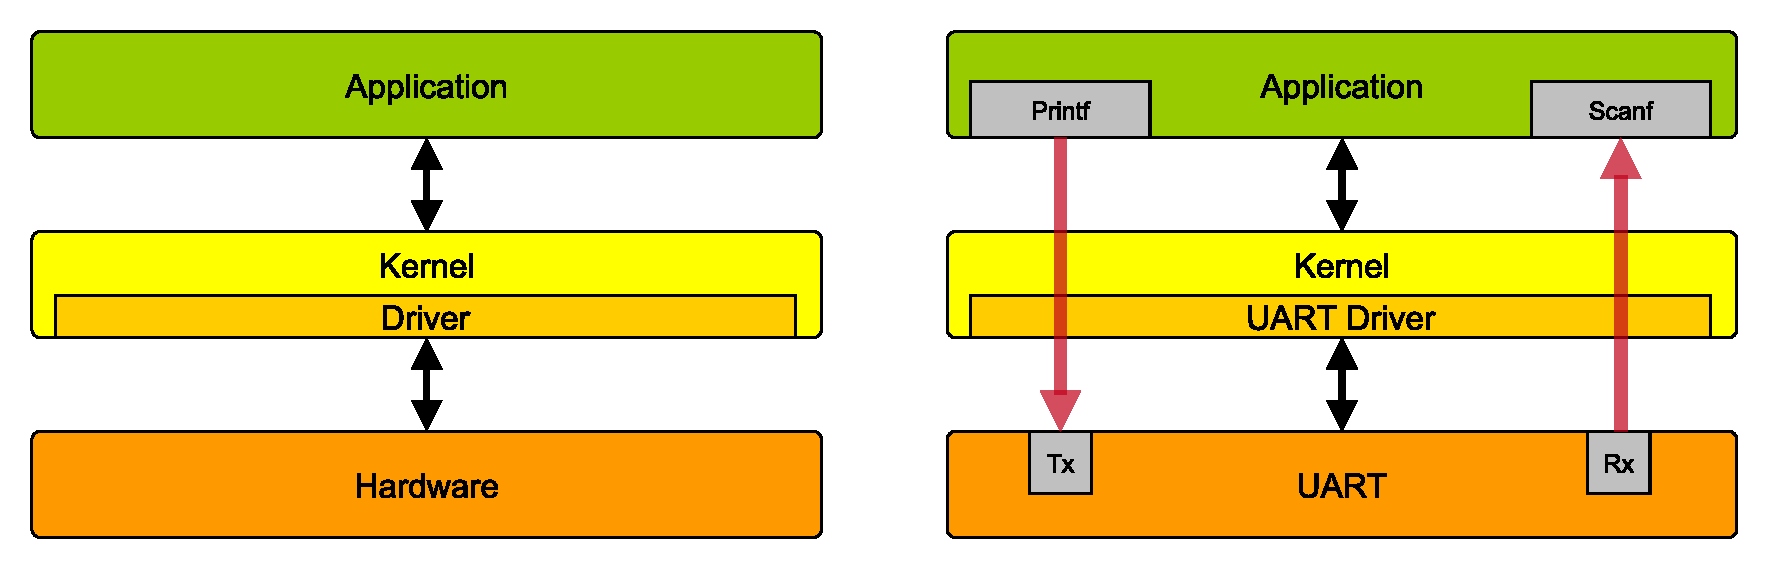
\includegraphics[width=\textwidth]{img/general/Kernel_Hardware_Layer.pdf}
\caption{Links:Kommunikation zwischen Applikation und Hardware.\\Rechts: Beispiel Kommunikation zwischen Applikation und UART über den Kernel.}
\label{figure_KernelHardwareLayer}
\end{center}
\end{figure}

\chapter{Anforderungsanalyse}
\label{chapter_Anforderungsanalyse}
Das Ziel dieser Arbeit ist es, einen Teststand entwickeln, der über die Messung der Degradation von optoelektronischen Sendern. Dadurch soll eine Qualifizierung der Bauelemente erfolgen. In diesem Kapitel wird zunächst das Szenario näher beschrieben und anschließend die sich daraus entwickelnden Anforderungen definiert.

\section{Szenario}
Ein Unternehmen stellt verschiedene optoelektronischen Sensoren her. Zur Sicherstellung der Zuverlässigkeit der verwendeten \acp{LED} sollen diese mittels eines automatisierten Teststandes bezüglich ihres Degradationsverhaltens qualifiziert werden.


\begin{figure}[H]
\begin{center}
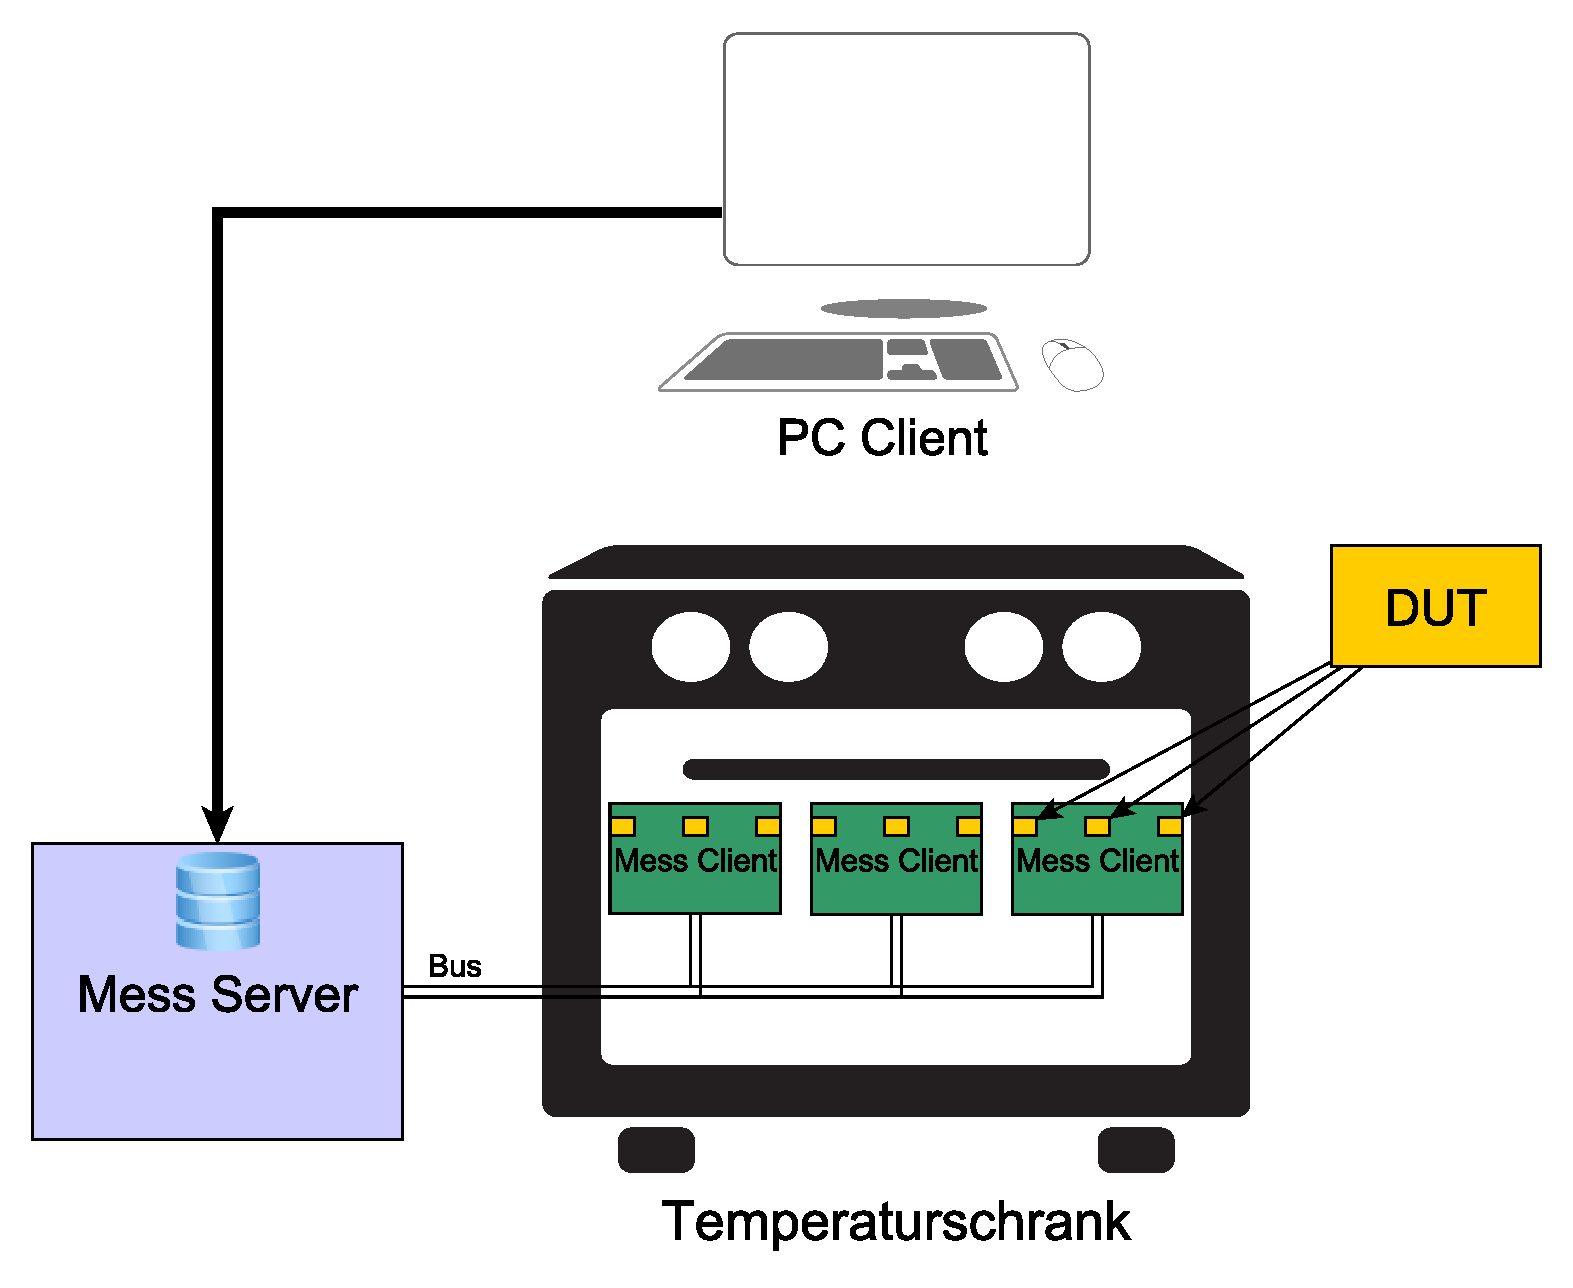
\includegraphics[width=0.6\textwidth]{img/general/Szenario.png}
\caption{Szenario}
\label{figure_Szenario}
\end{center}
\end{figure}

Der Teststand hat den in Abbildung \ref{figure_Szenario} zu sehenden Aufbau.
In einem Ofen befinden sich mehrere Mess-Clients. An diesen Mess-Clients sind jeweils 64 \acp{DUT} fest angeschlossen, bei denen das Degradationsverhalten aufgezeichnet werden soll.
Die Mess-Clients sind über einen Bus mit dem Mess-Server verbunden, welcher alle anfallenden Daten speichert.\\
Von einem PC-Client wird dann auf den Mess-Server zugegriffen um die Daten abzugreifen und grafisch auszuwerten.\\

\section{Analyse}

Die Akteure des Systems sind der Mess-Server, Mess-Client und PC-Client. Im Zuge dieser Arbeit soll der Mess-Server realisiert werden. Wobei die Interaktionsfähigkeit mit den anderen Akteuren sichergestellt werden muss.


\subsection{Mess-Client}
\label{section_Mess-Client}

Das Herzstück des Mess-Clients bildet ein STM8 8-Bit Mikrocontroller der Firma STMicroelectronics.
Auf jedem Mess-Client sind 64 \acp{DUT} befestigt. In zyklischen Abständen werden die Messdaten der Prüfobjekte aufgenommen und über eine RS232-Schnittstelle zur Verfügung gestellt.\\
Dieses System war zum großen Teil bereits gegeben, so dass lediglich die Übertragung der RS232 Schnittstelle geregelt werden musste. Dazu wurde ein Protokoll für die Kommunikation entworfen (sieht Abschnitt \ref{section_RS232_Protokoll}).
 
 \begin{figure}[!htb]
\minipage{0.48\textwidth}
  \includegraphics[width=\linewidth]{img/general/DegraBoardTop.jpg}
  \caption{Mess-Client Oberseite}\label{figure_DegraBoardTop}
\endminipage\hfill
\minipage{0.48\textwidth}%
  \includegraphics[width=\linewidth]{img/general/DegraBoardBottom.jpg}
  \caption{Mess-Client Unterseite}\label{figure_DegraBoardBottom}
\endminipage
\end{figure}


\textbf{------- Besondere RS232 chips, können RX hochohmig schalten. -------}


\subsection{Mess-Server}
\label{section_Mess-Server}

\begin{figure}[H]
\begin{center}
\includegraphics[width=0.6\textwidth]{img/general/BeagleBoneBlack.png}
\caption{BeagleBone Black}
\label{figure_Beagleboneblack}
\end{center}
\end{figure}


Als Mess-Server wird ein BeagleBone Black von Texas Instruments eingesetzt (siehe Abbildung \ref{figure_Beagleboneblack}). Dabei handelt es sich um einen kostengünstigen Einplatinencomputer mit offener Hardware. Damit ist es möglich, das BeagleBone Black auf individuelle Anforderungen anzupassen und selbst herzustellen. Auch gibt es eine große Community, die ständig die Entwicklung vorantreibt.
Er arbeitet mit einem AM335x 1GHz ARM® Cortex-A8 Prozessor, verfügt über 512MB DDR3 RAM und 4GB 8-bit eMMC internen Flash Speicher. Als Spannungsversorgung dient ein 5V 2A Netzteil.

Trotz der Kompaktheit des BeagleBone Black, bietet er ein ausreichendes Maß an Performance. Auf ihm kommt ein eingebettetes Debian-GNU/Linux Betriebssystem (sieht Abschnitt \ref{section_EmbeddedLinux}) zum Einsatz. Damit ist es möglich die umfangreichen Debian-Funktionen wie die Paketverwaltung zu nutzen. Es bietet auch den Vorteil, dass eine große Ähnlichkeit zu PC-Distributionen wie Ubuntu besteht und somit einfacher nutzbar ist (vgl. \cite{schroeder2009embedded}).\\
Außerdem sind Linux Mechanismen einfach nutzbar. So kann das RS232 Interface beispielsweise wie eine normale Datei beschrieben und gelesen werden.

Für die Kommunikation mit den anderen Akteuren im System, muss ein RS232 Bussystem und eine Ethernet Schnittstelle realisiert werden. Des Weiteren soll ein MySQL Datenbankserver auf dem Mess-Server die effiziente Verwaltung von Daten übernehmen.

\subsection{PC-Client}
\label{section_PC-Client}
Der PC-Client stellt eine Qt Desktopanwendung mit \ac{GUI} zur Auswertung der Messdaten.


\section{Anforderungen}

Folgende Anforderungen werden dabei an das System gestellt:
\begin{itemize}
\item Individuelle Parametrierung der \acp{DUT}
\item Automatische Erfassung der Messdaten
\item Fernzugriff auf den Mess-Server
\end{itemize}
\ \\
\textbf{Individuelle Parametrierung der \acp{DUT}}\\
Immer 64 \acp{DUT} befinden sich auf einem Mess-Client. Dabei sollen verschiedene Parameter für die \acp{DUT} berücksichtigt werden. 
Zum einen sollen die Intervalle in denen Messwerte aufgenommen werden konfigurierbar sein. Dies soll in mindestens 3 verschiedenen Intervallen möglich sein.

Beispiel: 

\begin{table}[H]
\begin{center}
\begin{tabular}{|l|l|}\hline
Zeitraum & Zeit zwischen Messungen \\ \hline
1. Woche & 12 Stunden\\ 
2. bis 4. Woche & 2 Tage\\ 

ab 5. Woche & 7 Tage\\ \hline
\end{tabular}
\caption{Intervalle}
\label{table_Intervalle}
\end{center}
\end{table}



Des Weiteren soll für jeden Mess-Client ein Pulsepattern definierbar sein. Dieses Pulsepattern wird dann als Versorgungssignal für die \acp{DUT} verwendet.

\textbf{Automatische Erfassung der Messdaten}\\
Die Messdaten der \acp{DUT} sollen zyklisch erfasst werden. Es soll die derzeitige Temperatur im Ofen, der gemessene Wert des Sensors und ein Zeitstempel gespeichert werden. Dabei sollen, wie bereits erwähnt, die Intervalle zwischen den Messungen konfigurierbar sein.\\
Für den einfachen und effizienten Zugriff auf die Daten, sollen diese in einer \ac{SQL} Datenbank abgelegt werden. Dafür ist eine Kommunikationsschnittstelle zwischen der Datenbank und den Mess-Clients erforderlich, welcher über den Mess-Server realisiert werden soll.

\textbf{Fernzugriff auf den Mess-Server}\\
Zur Auswertung der Messdaten, soll es möglich sein, von einem PC-Arbeitsplatz aus eine Verbindung zu dem Mess-Server aufzubauen. Die Messdaten sollen dann grafisch auf dem PC-Client zur Auswertung aufbereitet werden.
Auch soll ein Tunnelmodus direkten Zugriff von einem PC-Client auf einem Mess-Client ermöglichen. Dabei sollen die Parameter des Mess-Clients verändert werden können.


Diese Basis-Anforderungen und einige zusätzliche Anforderungen können wie in Tabelle \ref{table_Anforderungen} in funktionale und nicht-funktionale Anforderungen unterteilt werden.


\begin{table}[H]
\begin{center}
\begin{tabularx}{\textwidth}{|p{3cm}|X|X|X|}\hline
Art & Anforderung & Kommentar \\ \hline
Nicht-Funktional & Das System soll jederzeit verfügbar sein. & Bei Fehlern soll das System ohne große Ausfallzeit wieder Einsatzbereit sein. Zuverlässigkeit ist sehr wichtig.\\ \hline
Nicht-Funktional & Das Benutzerinterface soll zeitnah auf Anfragen reagieren. & Um Benutzerfreundlichkeit zu gewährleisten, soll auf Nutzeranfragen ohne lange Wartezeiten reagiert werden. \\ \hline
Funktional & Das System soll das Degradationsverhalten eines \ac{DUT} aufnehmen & Hauptanforderung des Systems. Messdaten sollen zu einem \ac{DUT} gesammelt werden, um den Grad der Degradation bestimmen zu können. \\ \hline
Funktional & Neue Mess-Clients sollen am PC-Client parametrierbar sein. & Parameter sollen auf dem Mess-Client und in einer Datenbank gespeichert werden. \\ \hline
Funktional & Neue bereits parametrierte Mess-Clients sollen automatisch in das System integrierbar sein. & Ein parametrierter Mess-Client kann direkt an den Bus im Ofen angeschlossen werden.\\ \hline
Funktional & Zyklische Erfassung von Messdaten. & Intervalle der Messdatenerfassung sind konfigurierbar.\\ \hline
Funktional & Messdaten sollen grafisch dargestellt werden. & Um die Daten auswerten zu können sollen sie grafisch aufbereitet werden.\\ \hline
Funktional & Die Messdaten sollen in einer Datenbank abgelegt werden. & Zum einfachen und effizienten Zugriff auf die Daten.\\ \hline
Funktional & Die Messdaten sollen via Fernzugriff erreichbar sein. & Von einem PC-Client aus, soll auf die Daten im lokalen Netzwerk zugegriffen werden können.\\ \hline
Funktional & Der Status des Systems soll ablesbar sein. & Über eine Anzeige soll das System lokal überwacht werden können.\\ \hline
Funktional & Nutzer Fehler sollen abgefangen werden. & Fehler bei der Bedienung durch den Nutzer sollen unterbunden werden.\\ \hline
\end{tabularx}
\caption{Anforderungen}
\label{table_Anforderungen}
\end{center}
\end{table}














\chapter{Konzept}
\label{chapter_Konzept}

Im folgenden Kapitel wird auf die Erstellung des Konzeptes eingegangen.

\section{Teststand}
\label{section_Teststand}

Das Gesamtsystem setzt sich aus drei Untersystemen zusammen:

\begin{itemize}

\item Mess-Client
\begin{itemize}
\item Übernimmt die lokale Ansteuerung der \acp{DUT}
\item Nimmt Messdaten auf und stellt sie zur Verfügung
\end{itemize}

\item Mess-Server
\begin{itemize}
\item Verwaltet angeschlossene Mess-Clients
\item Speichert alle Messdaten
\item Bildet das Bindeglied zwischen Mess-Client und dem PC-Client
\end{itemize}

\item PC-Client
\begin{itemize}
\item Parametriert die Mess-Clients
\item Wertet Messdaten aus und stellt sie leserlich da
\end{itemize}

\end{itemize}


\begin{figure}[H]
\begin{center}
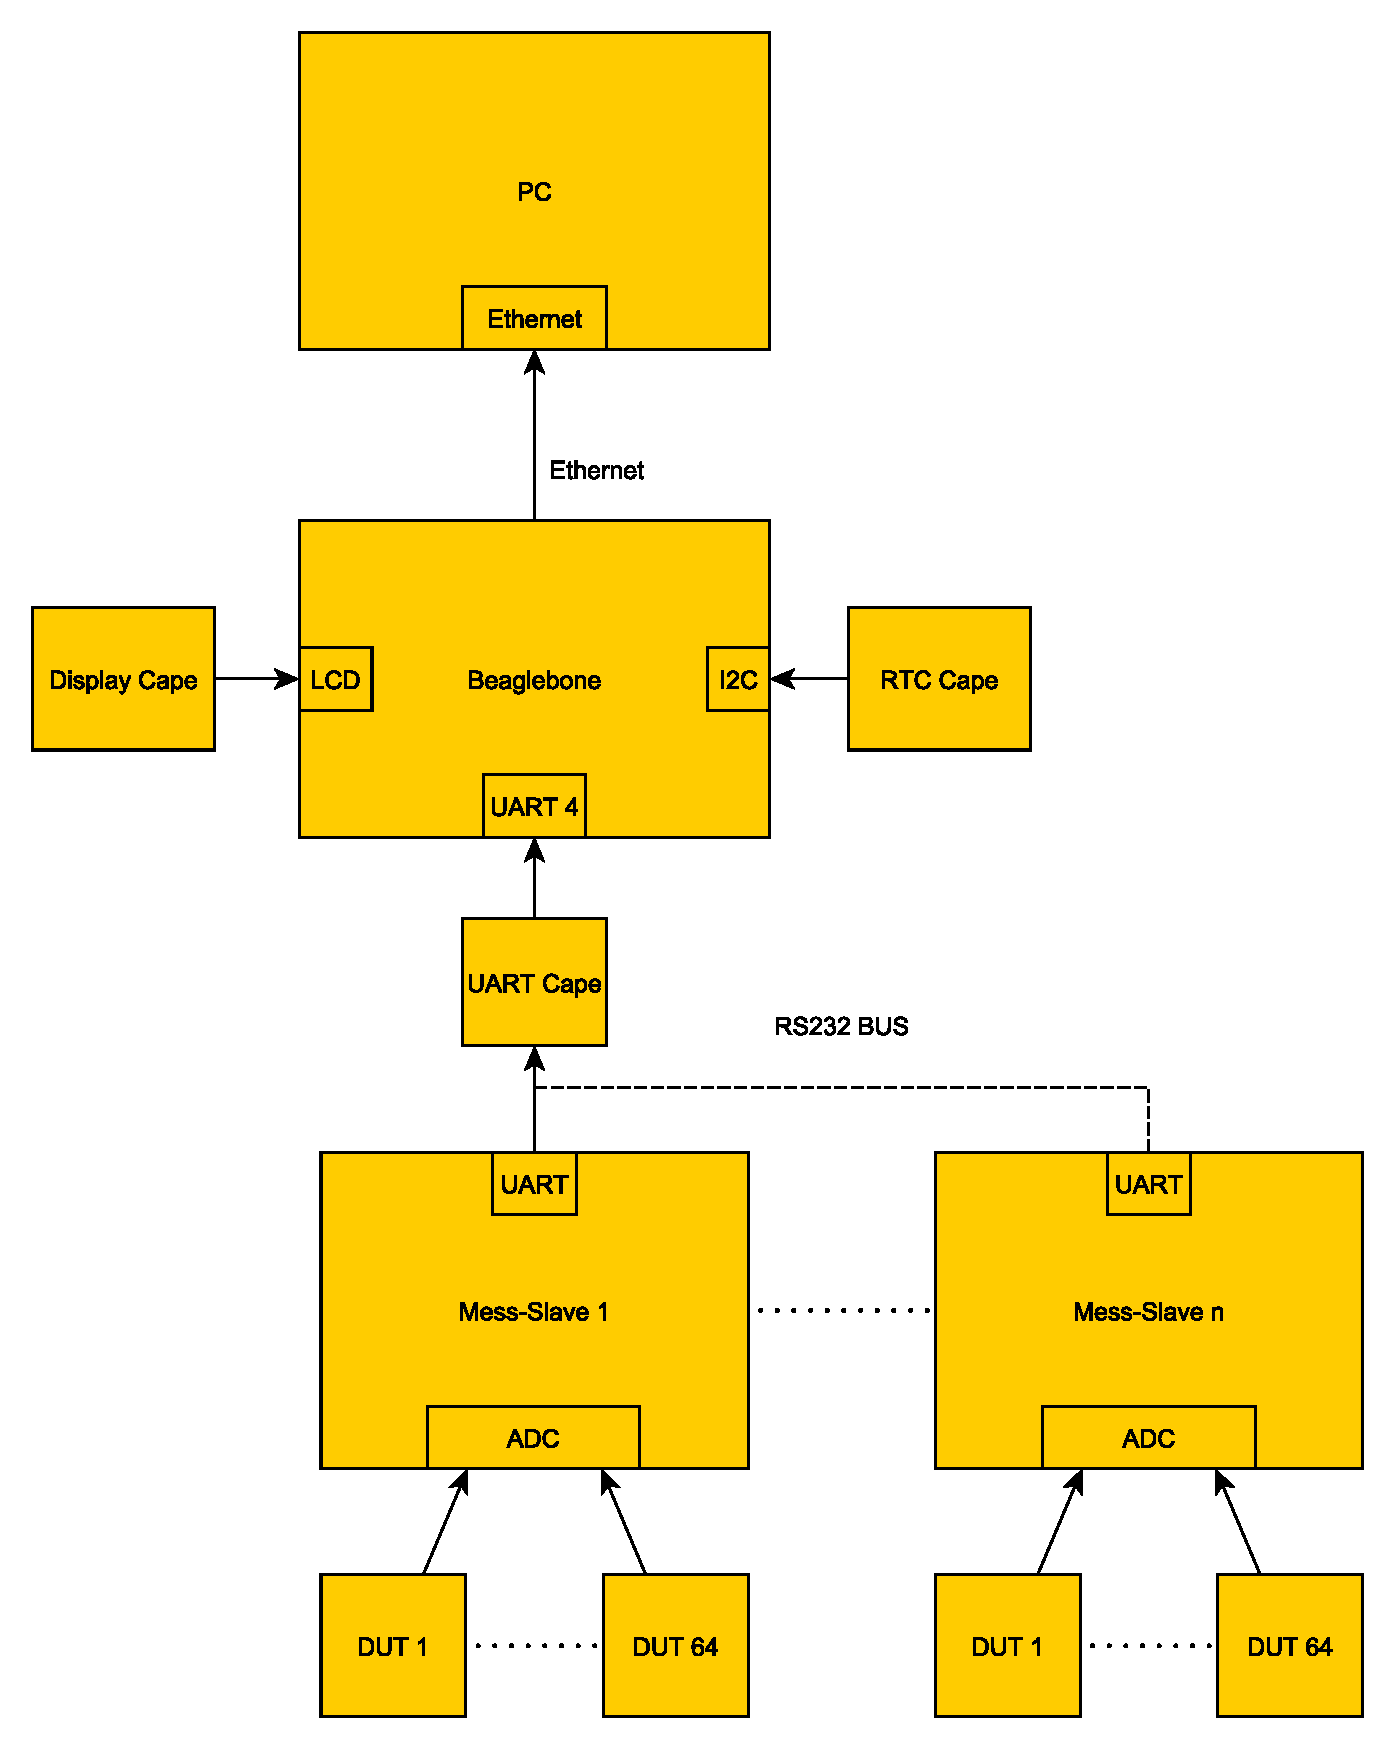
\includegraphics[width=\textwidth]{img/general/BlockPlan.pdf}
\caption{Gesamt System}
\label{Gesamt_System}
\end{center}
\end{figure}


\subsection{Mess-Client}
\label{section_Mess-Client}

Das Herzstück des Mess-Clients bildet ein STM8  8-Bit Mikrocontroller der Firma STMicroelectronics.
Auf jedem Mess-Client sind 64 \acp{DUT} befestigt. In zyklischen Abständen werden die Messdaten der Prüfobjekte aufgenommen und über eine RS232-Schnittstelle zur Verfügung gestellt (siehe Abbildung \ref{MessSlaveBlockPlan}.\\
Dieses System war zum großen Teil bereits gegeben, so dass lediglich die Übertragung der RS232 Schnittstelle geregelt werden musste. Dazu wurde ein Protokoll für die Kommunikation entworfen (sieht Abschnitt \ref{section_RS232_Protokoll}).
\\
%\begin{figure}[h]
%\begin{center}
%\includegraphics[width=\textwidth]{}
%\caption{Mess-Client Blockschaltplan}
%\label{MessSlaveBlockPlan}
%\end{center}
%\end{figure}


\subsection{Mess-Server}
\label{section_Mess-Server}

Als Mess-Server wird ein BeagleBone Black von Texas Instruments eingesetzt. Dabei handelt es sich um einen Einplatinen-Computer, der mit einem AM335x 1GHz ARM® Cortex-A8 Prozessor arbeitet. Das Betriebssystem ist eine Embedded Linux Debian Lösung.


\subsection{PC-Client}
\label{section_Verwaltung}
asdasad


\subsection{RS232 Protokoll}
\label{section_RS232_Protokoll}
Das Protokoll für die Kommunikation über die RS232 Schnittstelle ist nötig, um die Validität, Vollständigkeit und Zuverlässigkeit der Übertragungen sicherzustellen.\ \\

Folgende Kriterien sollen dabei erfüllt werden:
\begin{itemize}
\item Adressierung individueller Kommunikationspartner
\item Senden verschiedener Befehle
\item Variable Größe der Daten
\item Sicherstellung der Validität der Übertragung
\item Erweiterbar
\end{itemize}
\ \\

\subsubsection{Aufbau}
\begin{table}[H]
\begin{center}
\begin{tabularx}{\textwidth}{|X|X|X|X|c|X|}\hline
 1. Byte & 2. Byte & 3. Byte & 4. Byte & 5. Byte und folgend & Letztes Byte\\ \hline
  Adresse & Länge & Command & Subcommand & Nutzdaten & Checksumme\\ \hline
\end{tabularx}
\caption{Übertragungsrahmen}
\label{table_Frame}
\end{center}
\end{table}

Ein Rahmen besteht aus 4 Steuerbytes, 1 Checksummenbyte und maximal 30 Datenbytes. 

\textbf{1. Byte: Adresse \& Read/Write}

\begin{table}[H]
\begin{center}
\begin{tabularx}{\textwidth}{|X|X|X|X|X|X|X|X|}\hline
 7. Bit & 6. Bit & 5. Bit & 4. Bit & 3. Bit & 2. Bit & 1. Bit & 0. Bit\\ \hline
 R/W & Addr6 & Addr5 & Addr4 & Addr3 & Addr2 & Addr1 & Addr0\\ \hline
\end{tabularx}
\caption{1. Byte: Adresse \& Read/Write}
\label{table_1Byte}
\end{center}
\end{table}

Das erste Byte des Übertragungsrahmens setzt sich aus 7 Adressbits und einem Lese-/Schreibbit zusammen. Die ersten 7 Bits (Addr0 - Addr6) bilden die Adresse des anzusteuernden Mess-Clients. Daraus ergibt sich ein Adressraum von möglichen 128 Adressen, wobei Adresse 0 für neue Mess-Clients zur einmaligen Anmeldung im System reserviert ist.\\
Das höchste Bit ist das Lese-/Schreibbit. Der Mess-Client unterscheidet mithilfe dieses Bits, ob ein Befehl als Lese- oder Schreibzugriff interpretiert werden soll.\\

\begin{table}[H]
\begin{center}
\begin{tabular}{|l|l|}\hline
 R/W Bit & Beschreibung \\ \hline
 0 & Die Steuereinheit möchte lesen \\ \hline
 1 & Die Steuereinheit möchte schreiben \\ \hline
\end{tabular}
\caption{Read/Write}
\label{table_RW}
\end{center}
\end{table}


\textbf{2. Byte: Länge des Rahmens}

\begin{table}[H]
\begin{center}
\begin{tabularx}{\textwidth}{|X|X|X|X|X|X|X|X|}\hline
 7. Bit & 6. Bit & 5. Bit & 4. Bit & 3. Bit & 2. Bit & 1. Bit & 0. Bit\\ \hline
 Len7 & Len6 & Len5 & Len4 & Len3 & Len2 & Len1 & Len0\\ \hline
\end{tabularx}
\caption{2. Byte: Länge des Rahmens}
\label{table_2Byte}
\end{center}
\end{table}

Das zweite Byte gibt die Länge des gesamten Übertragungsrahmens inklusive Steuerbytes, Nutzdaten und Checksumme an.\\ Die minimale Länge eines Rahmens beträgt 5 Byte. Dabei handelt es sich um eine Übertragung ohne Nutzdaten und es werden lediglich die 4 Steuerbytes und das Byte für die Checksumme übertragen. Dies geschieht beispielsweise bei einer Leseanfrage.\\
Die maximale Länge eines Rahmen beträgt 35 Byte. Hierbei werden zusätzlich zu den 4 Steuerbytes und dem Byte für die Checksumme auch die maximale Nutzlast von 30 Byte übertragen. Dieser Fall kann beispielsweise bei Schreibzugriffen auftreten.


\textbf{3. Byte: Command}

\begin{table}[H]
\begin{center}
\begin{tabularx}{\textwidth}{|X|X|X|X|X|X|X|X|}\hline
 7. Bit & 6. Bit & 5. Bit & 4. Bit & 3. Bit & 2. Bit & 1. Bit & 0. Bit\\ \hline
 Cmd7 & Cmd6 & Cmd5 & Cmd4 & Cmd3 & Cmd2 & Cmd1 & Cmd0\\ \hline
\end{tabularx}
\caption{3. Byte: Command}
\label{table_3Byte}
\end{center}
\end{table}

Das dritte Byte repräsentiert den Befehl. Dieser gibt an, welche Aktion ausgeführt werden soll oder welcher Parameter angesprochen wird. 


\textbf{4. Byte: Subcommand}

\begin{table}[H]
\begin{center}
\begin{tabularx}{\textwidth}{|X|X|X|X|X|X|X|X|}\hline
 7. Bit & 6. Bit & 5. Bit & 4. Bit & 3. Bit & 2. Bit & 1. Bit & 0. Bit\\ \hline
 Scmd7 & Scmd6 & Scmd5 & Scmd4 & Scmd3 & Scmd2 & Scmd1 & Scmd0\\ \hline
\end{tabularx}
\caption{4. Byte: Subcommand}
\label{table_4Byte}
\end{center}
\end{table}

Das vierte Byte ist der Subcommand. Damit ist es möglich verschiedene Unterbefehle zu adressieren.


\textbf{5. Byte und folgend: Nutzdaten}

\begin{table}[H]
\begin{center}
\begin{tabularx}{\textwidth}{|X|X|X|X|X|X|X|X|}\hline
 7. Bit & 6. Bit & 5. Bit & 4. Bit & 3. Bit & 2. Bit & 1. Bit & 0. Bit\\ \hline
 Data7 & Data6 & Data5 & Data4 & Data3 & Data2 & Data1 & Data0\\ \hline
\end{tabularx}
\caption{5. Byte und folgend: Nutzdaten}
\label{table_5Byte}
\end{center}
\end{table}

Das fünfte Byte und die darauf folgendenx, tragen die Nutzdaten des Rahmens. 


\textbf{Letztes Byte: Checksumme}

\begin{table}[H]
\begin{center}
\begin{tabularx}{\textwidth}{|X|X|X|X|X|X|X|X|}\hline
 7. Bit & 6. Bit & 5. Bit & 4. Bit & 3. Bit & 2. Bit & 1. Bit & 0. Bit\\ \hline
 CKS7 & CKS6 & CKS5 & CKS4 & CKS3 & CKS2 & CKS1 & CKS0\\ \hline
\end{tabularx}
\caption{Letztes Byte: Checksumme}
\label{table_LastByte}
\end{center}
\end{table}

Das letzte Byte ist immer die Checksumme um sicherzustellen, dass alle Daten komplett und fehlerfrei übertragen wurden. Die Checksumme bildet sich dabei aus einer XOR Verknüpfung aller Bytes eines Übertragungsrahmens.

Beispiel:

Checksumme bilden:
 
1 xor 2 xor 3 xor 4 xor 5 = 1

Checksumme prüfen:

1 xor 2 xor 3 xor 4 xor 5 xor 1 = 0

\subsubsection{Commands und Subcommands}


\begin{table}[H]
\begin{center}
\begin{tabularx}{\textwidth}{|l|c|c|c|X|}\hline
 Command & Code & Subcommand & Datenbytes & Content Datatype\\ \hline
 ADC-Value & 0x00 & MUX-Kanal (0..63) & 2 & ADC Wert für spezifizierten Kanal \\ \hline
 Number Of Pulses & 0x04 & - & 1 & Anzahl der Pulse pro Pattern (0..50) \\ \hline
 Pulsewidth and -period & 0x05 & Pulsnummer & 4 & Pulsbreite und Pulseperiode \\ \hline
 Perform Pulseupdate & 0x06 & - & 0 &  \\ \hline
 DAC-value & 0x07 & - & 2 & DAC Wert \\ \hline
 Temperature & 0x08 & - & 1 & Wert des Temperatursensors \\ \hline
 LTT name & 0x09 & - & 1..30 & Name \\ \hline
 Rs232-Address & 0x0A & - & 1 & Adresse \\ \hline
 Error & 0x0B & MUX-Channel (0..63) & 2 & ADC Value for specified Channel \\ \hline
 Measurement Intervall & 0x0C & Intervallnummer (0..2) & 4 & Minutenabstand zwischen den Messungen + Tagesabstand zum nächsten Interval \\ \hline
\end{tabularx}
\caption{Befehlsliste}
\label{table_Commands}
\end{center}
\end{table}



\section{Datenbank}
\label{section_EntwurfDatenbank}

Aus den Anforderungen ergibt sich folgendes \ac{ERM} (siehe Abbildung \ref{ERM}). \\

\begin{figure}[H]
\begin{center}
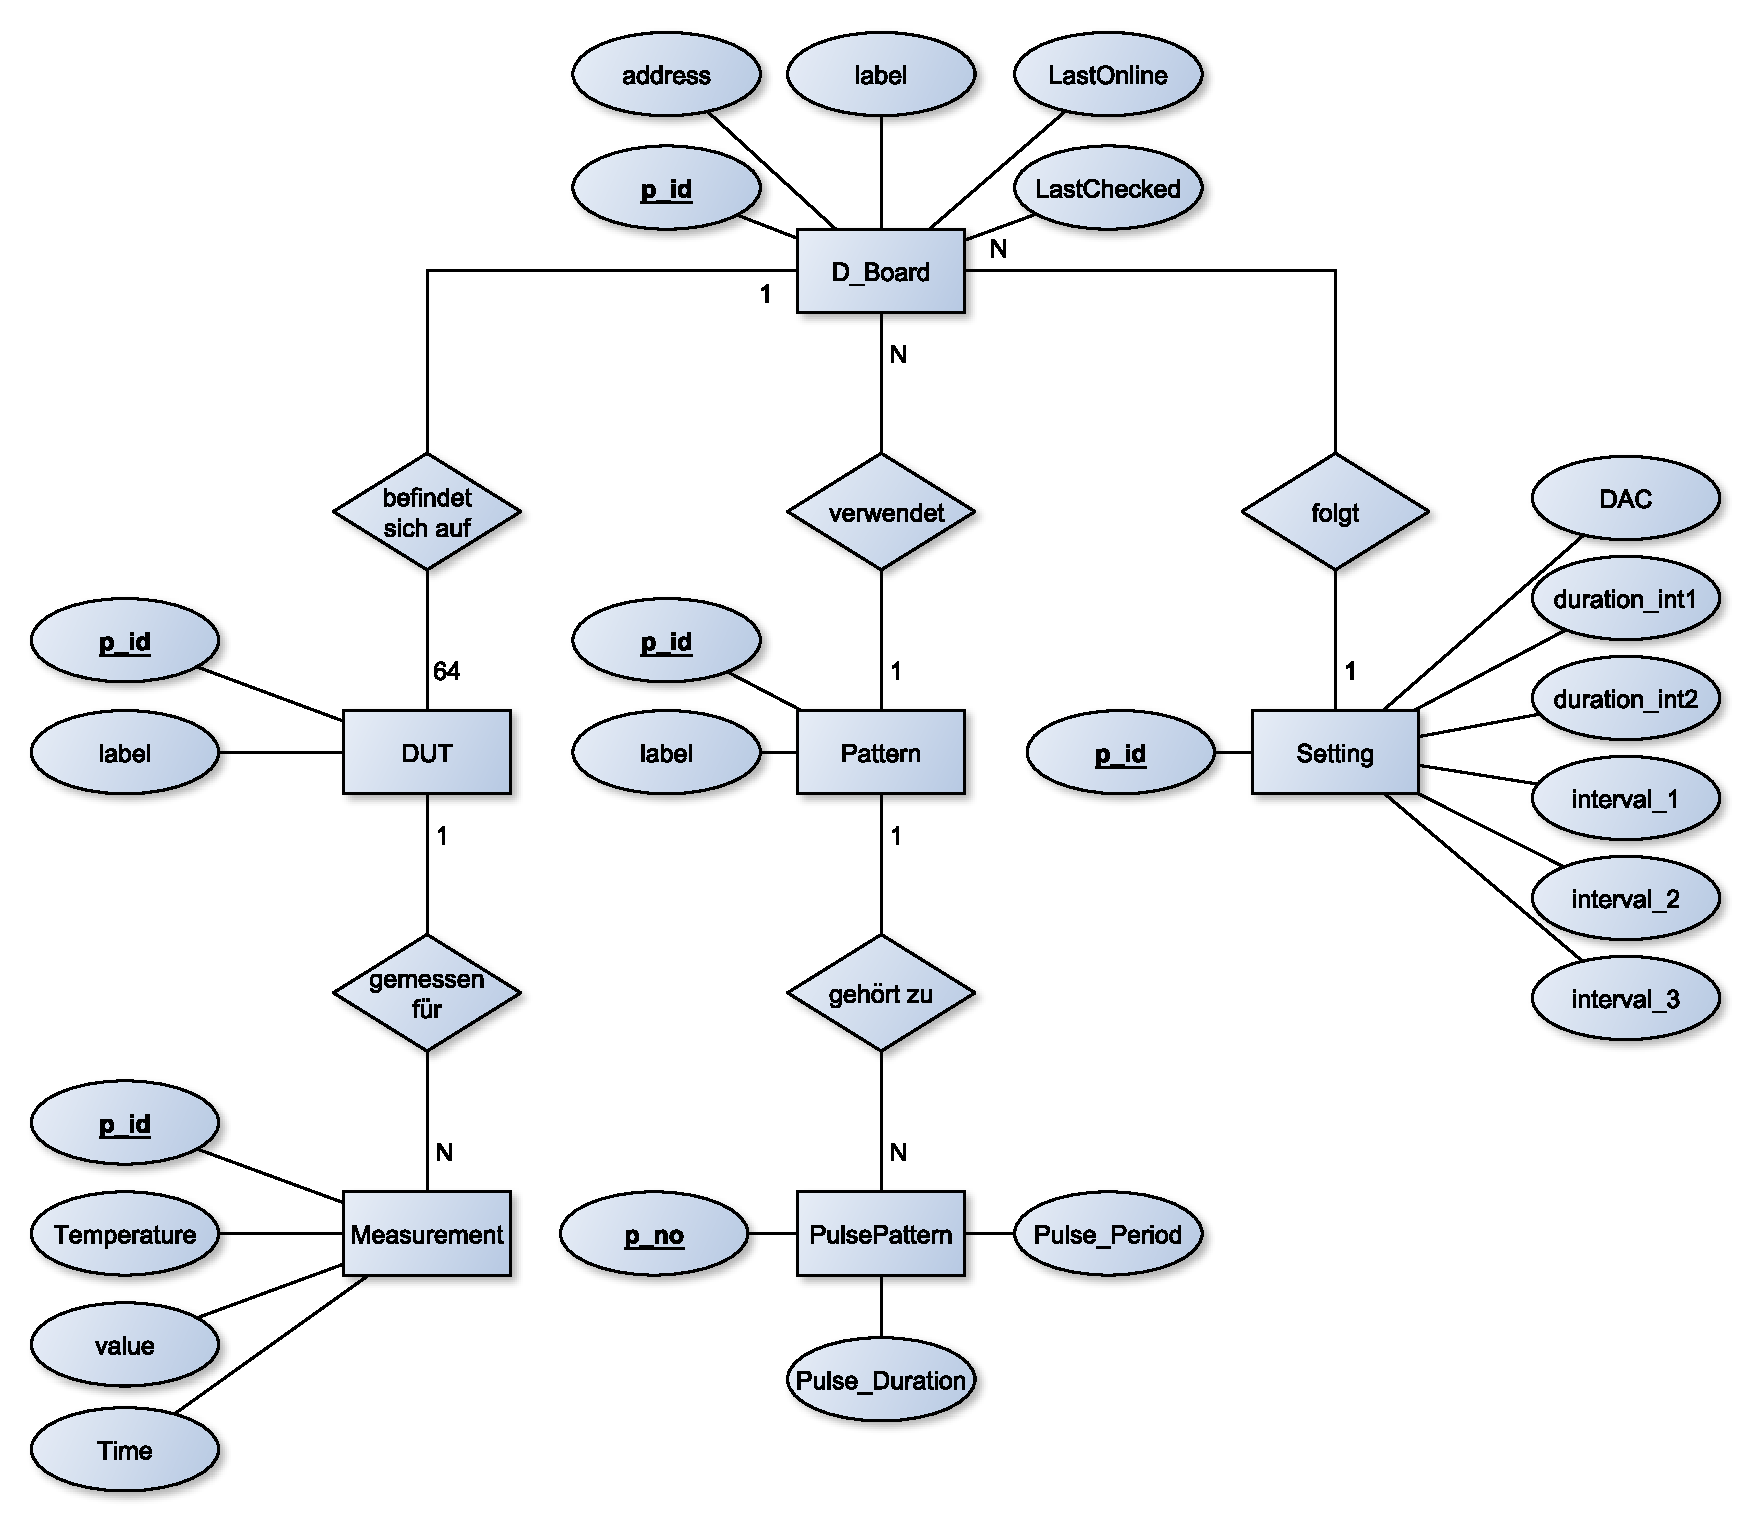
\includegraphics[width=\textwidth]{img/general/ER_Diagramm.pdf}
\caption{Entity Relationship Modell}
\label{ERM}
\end{center}
\end{figure}


Die Datenbank muss folgende Daten für die Parameter der Mess-Clients aufnehmen:\\

\begin{table}[H]
\begin{center}
\begin{tabular}{|l|l|}\hline
Parameter & Beschreibung \\ \hline
DAC & Vorverstärkung\\ 
duration\_int1 & Dauer der Zeit die Werte im 1.Interval aufgenommen werden in Tagen\\ 
duration\_int2 & Dauer der Zeit die Werte im 2.Interval aufgenommen werden in Tagen\\ 
interval\_1 & Abstand zwischen den Messungen im 1. Interval in Minuten\\ 
interval\_2 & Abstand zwischen den Messungen im 2. Interval in Minuten\\ 
interval\_3 & Abstand zwischen den Messungen nach dem 2. Interval in Minuten\\ \hline
\end{tabular}
\caption{Tabelle Setting}
\label{table_TabelleSetting}
\end{center}
\end{table}





\chapter{Implementieruung}
\label{chapter_Implementierung}

\section{Hardware}

\section{Software}

tcp server event gestuert

rs232 timeouts messdatenerfassung

\chapter{Testen und Validieren}
\label{chapter_Testen_und_Validieren}

Da das System in einem Langzeit-Teststand eingesetzt werden soll, ist die Zuverlässigkeit und die Betriebsfähigkeit über lange Zeiträume besonders wichtig. Es darf keine großen Performanceeinbußen oder lange Ausfälle beim Betrieb geben. In diesem Kapitel wird auf die Tests zur Sicherstellung dieser Kriterien eingegangen.

\section{Speicherlecks}

Ein häufiger Grund für Performanceeinbußen sind Speicherlecks (englisch: memory leak). Speicherlecks sind Fehler in der Programmierung der Speicherverwaltung, wodurch Speicher belegt, aber ungenutzt ist und nicht wieder freigegeben wird. Dabei kommt es zu einer immer größer werdenden Speichernutzung, bis der gesamte Speicher des Systems ausgelastet ist und es sich stark verlangsamt oder sogar Abstürzt.\\
Um Speicherlecks auszuschließen wurde die Steuerungssoftware mittels Valgrind \cite{valgrind} auf Speicherfehler überprüft. Dabei wurden alle Speicherlecks behoben.\\

\section{Stromausfall}

Nach einem Stromausfall muss das System binnen kürzester Zeit wieder einsatzbereit sein. Zur Sicherstellung dieser Eigenschaft wurden 20 Stromausfälle durch trennen und anschließend erneute verbinden der Stromversorgung simuliert.\\
Bei 20 Versuchen ist das System ohne Probleme 

\section{Testaufbau}

Im Testaufbau werden zwei Mess-Clients an einen Mess-Server angeschlossen
\chapter{Fazit und Ausblick}
\label{chapter_FazitUndAusblick}
sicherheit mysql verbindung, webinterface maybe

Lokale ausgabe messdaten für bestimmtes board über micro sd card

Jedoch entstehen dadurch Sicherheitsrisiken, da lediglich die Benutzername und Passwort Kombination einen Schutz gegen unerlaubten Zugriff bietet. Außerdem existieren keine Restriktionen für die Anfragen die an den MySQL Server gestellt werden können, wodurch die Daten gefährdet sind.
%%%
%%
%
%%%%%%%%%%%%%%%%%%%%%%%%%%%%%%%%%%%%%%%%%%%%%%%%%%%%%%%%%%%%%%%%%%%%%%%%%%%%%%%%%%%%%%%%%%%%%%%%%%%%%%%%%%%%%%%%%%%%
%%%%%%%%%%%%%%%%%%%%%%%%%%%%%%%%%%%% ENDE der wissenschaftlichen Arbeit %%%%%%%%%%%%%%%%%%%%%%%%%%%%%%%%%%%%%%%%%%%%
%%%%%%%%%%%%%%%%%%%%%%%%%%%%%%%%%%%%%%%%%%%%%%%%%%%%%%%%%%%%%%%%%%%%%%%%%%%%%%%%%%%%%%%%%%%%%%%%%%%%%%%%%%%%%%%%%%%%
%
%%
%%%
%\protect \addtocontents{toc}{\protect\newpage}  	% Seitenumbruch im Inhaltsverzeichnis
\clearpage
%
%%% Abschlussbetrachtung / Ausblick
\include{part/04_abschlussbetrachtung}
%
\clearpage \pagenumbering{roman}
%
%\pagestyle{plain}									% Seitenlayout (Standard) mit zentrierter Seitennummerierung				!!! ÜBERFLÜSSIG???!!!
%
%### Kapiteltitel auf Standardlayout zurücksetzen
\titleformat{\chapter}[display]{\normalfont\huge\bfseries}{\chaptertitlename\ \thechapter}{20pt}{\Huge}
%###%
%
%%%%%%%%%%%%%%%%%% L I T E R A T U R V E R Z E I C H N I S & A N H A N G %%%%%%%%%%%%%%%%%%%%%%%%%%
%
%\part{Literatur und Anhang}
%\label{part_anhang}
%\interlinepenalty = 10000
%
%%% Literaturverzeichnis, mit BibTeX
%
\phantomsection \addcontentsline{toc}{chapter}{Literaturverzeichnis}
\nocite{*} 										% auch die nicht verwendeten bibtex-Einträge einblenden
\bibliography{Literatur}
%
\clearpage
\include{appendix/appendix}
%\include{part/05_bib_appendix}
%%%
%
% Schmutzblatt (leere Seite am Ende)
%
\newpage                                    
\pagestyle{empty}
\begin{figure}[H]
\centering
%\includegraphics[width=0.9\textwidth]{pix/general/leer.png}
\end{figure}
%
\end{document}
%
%%% CODE - ARCHIV %%%
%\let\origitemize\itemize							% Zeilenabstand in \itemize-Umgebung global verringern
%\def\itemize{\origitemize\itemsep-7pt}
%